\section{Introduction}
The observed range of bacterial growth rates is enormously diverse. In
natural environments, some microbial organisms may double only once per
year \citep{mikucki2009} while in comfortable laboratory conditions, growth
can be rapid with several divisions per hour \citep{schaechter1958}. This six
order-of-magnitude difference in time scales of growth encompasses different microbial
species and lifestyles, yet even for a single species such as \textit{Escherichia
coli}, the growth rate can be modulated over a comparably large scale by tuning the
type and amount of nutrients in the growth medium \citep{liu2005a}. This remarkable
plasticity in growth rate illustrates the intimate relationship between
environmental conditions and the rates at which cells convert nutrients into
new cellular material -- a relationship that has remained a major topic of
inquiry in bacterial physiology for over a century \citep{jun2018}.

% Jacques Monod once remarked that ``the study of the growth of bacterial
% cultures does not constitute a specialized subject or branch of research, it
% is the basic method of Microbiology.’’ Those words ring as true today as they
% did when they were written 70 years ago \citep{monod1949} with the
% quantitative power of this "method" recently undergoing renaissance. Many of
% the key questions addressed by the pioneering efforts in the middle of the
% last century can be revisited by examining them through the lens of the
% increasingly refined molecular census that is available for bacteria such as
% the microbial workhorse \textit{E. coli}.

One of the key insights of the past 70's years was the discovery of bacterial "growth laws" \citep{schaechter1958}, 
empirical relationships relating the bacterial growth rate to the protein and RNA composition 
of the intracellular milieu. Over the past decade, a flurry of work \citep{molenaar2009, scott2010,
klumpp2014, basan2015, dai2016, erickson2017} have examined these growth laws at
a quantitative level, developing a series of mathematical models from which 
the growth laws naturally emerge. However, these models are highly phenomenological and 
lack a concrete connection to the molecular details of how the various macromolecules function 
and how they are regulated. Conversely, the "molecular revolution" in biology has 
yielded an impressive collection of precise measurements of the rates, durations, and 
turnovers of myriad biochemical reactions \textit{in vivo}, \textit{in vitro}, and \textit{in silico} \citep{davidi2016a}. 
Despite this mountain of quantitative data at the molecular (and frequently atomic) level,
it remains difficult to understand at a quantitative level how these reaction networks and the 
copy numbers of its enzymatic constituents conspire to yield macro-scale phenomena such as a well-defined
bacterial growth rate. In this work, we use recent proteomic data sets 
from \textit{E. coli} to quantitatively relate these two resolutions of understanding.

Several of the evergreen questions about bacterial growth and physiology that
were originally raised by microbiologists in the middle of the 20th century
can now be reframed in light of this newly available proteomic data. For example, what
biological processes are the primary determinants for how quickly bacterial
cells can grow and reproduce? Why do cells modulate the absolute numbers and
relative ratios of their molecular constituents as a function of changes in
growth rate or nutrient availability? In this paper, we begin by considering
these two questions from two distinct angles. First, as a result of an array
of high-quality proteome-wide measurements of \textit{E. coli} under diverse
growth conditions, we have a census that allows us to explore how the number
of key molecular players change as a function of growth rate. Here, we have
assembled a singular data set using measurements collected over the past
decade via mass spectrometry \citep{schmidt2016, peebo2015, valgepea2013} or
ribosomal profiling \citep{li2014} of the composition of the \textit{E. coli}
proteome across 36 unique growth rates (see the Appendix Section
"\nameref{sec:SI_exp_summary}" for a further discussion of the data). Second,
by compiling molecular turnover rate measurements for many of the fundamental
processes associated with bacterial growth, we make quantitative estimates of
a handful of key cellular processes (schematized in \FIG{categories}) to determine whether
our current understanding of the dynamics of these processes are sufficient
to explain the magnitude of the observed protein copy numbers across
conditions (see \BOX{estimate_rules} describing the philosophy behind this
approach). The census, combined with these estimates, provide a window into
the question of whether the rates of central processes such as energy
generation or DNA synthesis vary systematically as a function of
cell growth rate by altering protein copy number.

Throughout our estimates, we consider an archetypal growth rate of $\approx$ 0.5
hr$^{-1}$ corresponding to a doubling time of $\approx$ 5000 seconds, as the
data sets examined here heavily sample this growth regime. While we formulate
point estimates for the protein abundances at this division time, we also
consider how these values will vary at other growth rates due to changes in cell
size, surface area, and chromosome copy number \citep{taheriaraghi2015,
harris2018}. For the majority of the processes considered, we find that the
protein copy numbers appear tuned for the task of cell doubling across a
continuum of growth rates. Thus, our understanding of the kinetics of various
biological processes is sufficient to quantitatively explain the observed
abundances of these proteins.

From these estimates, it emerges that translation, particularly the synthesis
of ribosomal proteins, is a plausible candidate that limits the rate of cell
division in \textit{E. coli}. We reach this conclusion by considering that
ribosome synthesis is 1) a rate limiting step for the \textit{fastest}
bacterial division, and 2) a major determinant of bacterial growth across the
nutrient conditions we have considered under steady state, exponential
growth. This enables us to suggest that the long-observed correlation between
growth rate and cell size \citep{schaechter1958, si2017} can be simply
attributed to the increased absolute number of ribosomes per cell under
conditions supporting extremely rapid growth. To better understand how the
observed alterations in absolute protein abundances, and in particular,
changes in ribosome copy number, influence growth rate across different
nutrient conditions we consider a minimal model of cellular growth. Our
conclusions from these analyses provide important insight into how \textit{E.
coli} regulates growth across conditions of differing nutrient availability
and identifies fundamental constraints in bacterial growth more broadly.

\begin{figure}
    \centering{
    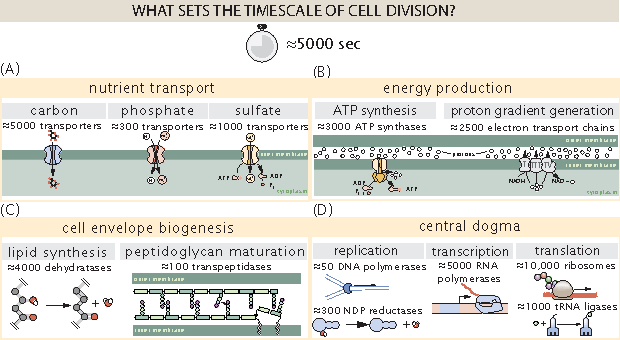
\includegraphics{main_figs/schematic_categories_grouped.pdf}
    \caption{\textbf{Transport and synthesis processes necessary for cell division.}
            We consider an array of processes necessary for a cell to double its
            molecular components, broadly grouped into four classes. These
            categories are (A) nutrient transport across the cell membrane, (B) cell envelope
            biogenesis, (C) energy production (namely, ATP synthesis), and (D) processes associated with the central dogma.
            Numbers shown are the approximate number of complexes of each type
            observed at a growth rate of 0.5 hr$^{-1}$, or a cell doubling time
            of $\approx$ 5000 s.}
    \label{fig:categories}
    }
\end{figure}
